El enunciado presenta el problema de hallar el camino entre 2 puntos que se recorra en el menor tiempo posible, dandonos un escenario en donde los caminos presentan paredes que podemos atravezar rompiendolas, teniendo a la vez, una determinada cantidad de rupturas a poder realizar. La solución buscada será entre todos los caminos posibles desde el origen al destino, el que sea mínimo.

Cada camino esta compuesto de unas unidades "caminables", que las llamaremos baldozas. Ir de una baldoza a otra consume la misma cantidad de tiempo en todos los casos. Por otro lado, hay 
baldozas que demandan romper una pared para ser caminadas, con lo cual el camino que se esta transitando debe gastar 1 unidad de esfuerzo en romperla, factor que no influye en el tiempo del recorrido.

Si caracterizamos cada baldoza con un nodo, y la posibilidad de ir de una baldoza a otra como una arista, entonces podemos modelar el problema con un grafo. Como el factor tiempo es constante en cada traslado entre baldozas, las aristas tendrán todas el mismo valor.

A partir de este grafo, sacar el camino mínimo del nodo origen al destino se puede realizar utilizando el algoritmo de busqueda por anchura, el cual permite saber la distancia (o tiempo) a la que se encuentran de determinado nodo cada uno de los demas. De aplicarlo sobre la estructura propuesta en forma directa, se obtendrían soluciones invalidálidas, ya que es necesario tener en cuenta la restricción de cantidad de paredes para romper. También se puede ver que el algoritmo solo, no considera todos los posidbles caminos válidos hacia el destino, con lo que se pierden soluciones validas, al restringir el uso de cada nodo a 1 solo camino:

  \vspace*{0.3cm} \vspace*{0.3cm}
  \begin{center}
 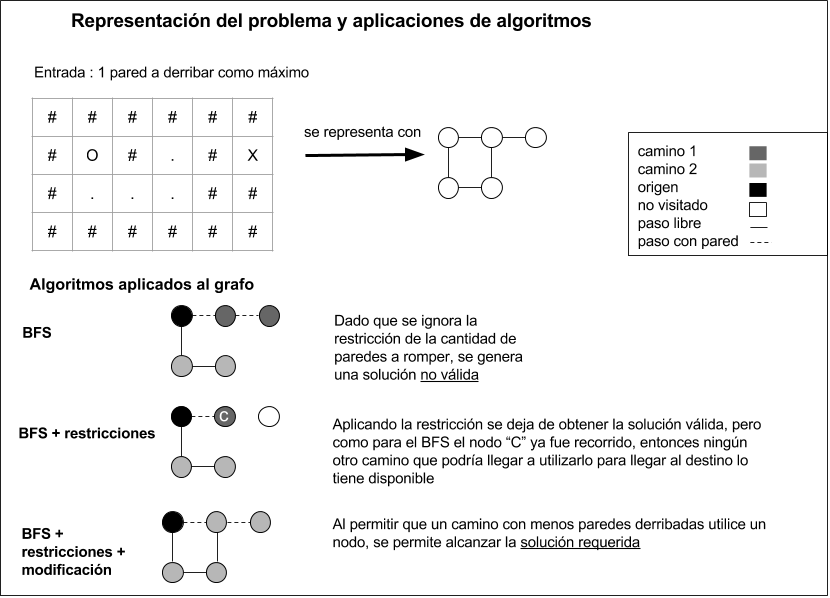
\includegraphics[scale=0.6]{./EJ1/ej1-explicacion.png}
  \end{center}
  \vspace*{0.3cm}

Para poder calcular todos los caminos que pueden llegar efectivamente al destino, en cada nodo se guardará las caracteristicas de tiempo y paredes necesarias para alcanzarlo:
\begin{itemize}
\item Si no ha sido alcanzado, entonces, se guarda el estado en el que se encuentra el nodo desde donde hacemos la visita: si se atravezo una o más paredes para lograrlo, se marca en su estado, al igual que el tiempo insumido en alcanzarlo.
\item Si ya ha sido alcanzado, entonces si la cantidad de paredes rotas hasta llegar hasta él desde el nodo actual es menor a la cantidad de paredes que fueron rotas anteriormente, entonces sin tener en cuenta el tiempo previo, se considera que el camino actual es la mejor forma de alcanzar al nuevo nodo, guardando los datos del camino actual en el nodo.
\item En el caso de que alcanzar al nodo previamente visitado, demande el mismo tiempo y esfuerzo que en el camino actual, se desestima el camino actual.
\item Si el nodo a evaluar es el destino, se da por finalizado el algoritmo y se devuelve el estado del camino que lo alcanzó.
\end{itemize}